\chapter{ARTS, the Atmospheric Radiative Transfer Simulator}
\label{sec:concept}

\starthistory
090424 & Complete revision and new text by Patrick Eriksson.\\
080729 & Section on command line parameters updated by Stefan Buehler.\\
020613 & Updated and extended by Stefan Buehler.\\
000616 & ARTS concept described by Stefan Buehler. \\
\stophistory

\graphicspath{{Figs/concept/}}


This section introduces and describes the basic ideas underlying the
ARTS programme. It also presents some terminology. You should read
it if you want to understand how the program works and how it can be
used efficiently.



\section{What is ARTS?}
%
The Atmospheric Radiative Transfer Simulator, ARTS, is an atmospheric
forward model. That is, a software for performing simulations of
atmospheric radiative transfer. ARTS is a relatively general and
flexible forward model, where a basic aim is to provide a platform
where new calculation features easily can be added. However, the
development of ARTS was initiated to deal with passive mm and sub-mm
measurements. Emission generated in the atmosphere or by the Earth's
surface is here detected. IR radiation is governed by the same basic
physical principles and this wavelength region is also well
handled. In fact, ARTS contains so far no dedicated methods for
scattering of solar radiation and there is basically a restriction to
simulations of longwave radiation.

The main application of ARTS should be to perform retrievals around
atmospheric measurements. A special feature of ARTS is also a high
flexibility when defining observation geometry (including scanning
features) and sensor characteristics. Jacobians are also provided (see
below). Though, the core task of the retrievals is to handle the
atmospheric radiative transfer and ARTS can also be used for basic
studies of atmospheric radiations
\citep{buehler:recen:06,john:under:06}.

There exist two versions of ARTS. This user guide deals with the later
of the two versions, here denoted as just ARTS. ARTS-1, the first
version of ARTS \citep{buehler:artst:05} can only handle 1D
atmospheres with unpolarised radiation and situations where scattering
can be neglected. These restrictions have been removed to this
version. A short summary of ARTS's main features:
\begin{description}
\item[The atmosphere] can be 1D, 2D or 3D. That is, atmospheric
  variables (temperature, gas concentrations etc.) can be assumed to
  only vary in the vertical dimension (1D), to have no longitude
  variation (2D) or vary in all three spatial dimensions (3D).
\item[The surface] and the geoid can have arbitrary shapes. That is,
  there are no limitations to a flat or spherical surface.
\item[Polarisation] is fully described by using the Stokes formalism.
\item[Scattering] can be considered by two modules, DOIT
  (Section~\ref{sec:scattering}) and MC
  (Section~\ref{sec:montecarlo}). The scattering calculations are for
  efficiency reasons confined to a region of the atmosphere denoted as
  the cloud box.
\item[Observation geometry] is free. That is, the forward model can be
  used to simulate ground-based, down-looking, limb sounding and
  balloon/aircraft measurements.
\item[Sensor characteristics] can be incorporated in a flexible and
  efficient manner.
\item[Jacobians,] the partial derivatives of simulated measurement
  with respect to forward model variables, can be provided for a
  number of variables, where analytical expressions are used as far as
  possible.
\end{description}
Details are found in later parts of the user guide. Use the table of
contents and the index for navigating through the user guide.



\section{Documentation guide}
%====================
\label{sec:concept:doc}

If you are totally new to ARTS and look for an introduction, we can
not yet offer any dedicated reading beside this section. The ambition
is to write an ARTS journal article during 2009. Many basic features
are common between ARTS-1 and ARTS, and \citet{buehler:artst:05}
introducing ARTS-1 is relevant also for this ARTS version and should
be worthwhile reading.

The main documentation sources for ARTS are the on-line documentation
and control file examples. The on-line documentation is described in
Section ~\ref{sec:concept:comline}. ARTS comes with a set of control
files that have two purposes: (1) To allow testing of the code at each
commit, (2) To act as practical examples for new users. These control
files are found in the \verb|tests/| sub-folder. Please, note that the
include mechanism (Section~\ref{sec:concept:envvars}) is used heavily,
where files from the \verb|includes/| sub-folder are selected.

Algorithms and details of the calculations are described by this user
guide. The user guide is fairly extensive, but due to a lack of direct
funding for this work it is not possible for us to reach a complete
coverage. All help to make this user guide more complete is highly
appreciated. For some parts of ARTS we refer to journal articles:
\begin{itemize}
\item The calculation approach for incorporation of sensor
  characteristics is described by \citet{eriksson:06}.
\item The Discrete Ordinate Iterative method (DOIT) for handling scattering
  is presented in \citet{emde04:_doit_jgr}.
\item \citet{davisetal:04} describe the Monte Carlo scattering method
  implemented in ARTS.
\end{itemize}



\section{Command line parameters}
%=================================
\label{sec:concept:comline}

ARTS offers a number of useful \textindex{command line parameters}. In
general, there is a short form and a long form for each parameter. The
short form consists of a minus sign and a single letter, whereas the
long form consists of two minus signs and a descriptive name.

\subsection*{Help}
%
To get a full list of available command line parameters, type
\begin{quote}
\begin{verbatim}
  arts -h
\end{verbatim}
\end{quote}
or
\begin{quote}
\begin{verbatim}
  arts --help
\end{verbatim}
\end{quote}


\subsection*{Include files}
%
See Section~\ref{sec:concept:envvars}.


\subsection*{Online documentation}
%
Most useful at the beginning should be the \artsstyle{-d}
(\artsstyle{--describe}), \artsstyle{-m} (\artsstyle{--methods}), \artsstyle{-w}
(\artsstyle{--workspacevariables}), and \artsstyle{-i} (\artsstyle{--input}) flags.
For instance, the \artsstyle{-d} (\artsstyle{--describe}) flag gives you online
documentation for any workspace method or workspace variable. Usage:
\begin{quote}
\begin{verbatim}
  arts -d f_grid
\end{verbatim}
\end{quote}
will print documentation about the workspace variable \artsstyle{f\_grid}, which
happens to be the monochromatic frequency grid.

But what methods and variables are available? You can find out by
typing
\begin{quote}
\begin{verbatim}
  arts -m all
\end{verbatim}
\end{quote}
which will list all workspace methods, or by typing 
\begin{quote}
\begin{verbatim}
  arts -w all
\end{verbatim}
\end{quote}
which will list all workspace variables. As you can see, these lists
are quite long. But you can get more specific information:
\begin{quote}
\begin{verbatim}
  arts -m f_grid
\end{verbatim}
\end{quote}
will give you a list of all methods that can generate the workspace
variable \artsstyle{f\_grid}. Specific and generic methods are listed
separately. Generic methods are in this case all methods producing a
Vector, since \artsstyle{f\_grid} belongs to this group. A similar task is
performed by the \artsstyle{-i} (\artsstyle{--input}) flag, with the difference
that \artsstyle{arts -i f\_grid} will list those methods that require
\artsstyle{f\_grid} as \emph{input}, whereas \artsstyle{arts -m f\_grid} lists
those that produce \artsstyle{f\_grid} as output. Finally,
\begin{quote}
\begin{verbatim}
  arts -w abs_coefCalc
\end{verbatim}
\end{quote}
will give you all variables required by the method \artsstyle{abs\_coefCalc}
(the variable \artsstyle{f\_grid} happens to be one of them).

Using these command line parameters, it is easy to build up a
control file. The trick is, to start at the end. Say you want to
compute absorption coefficients. First of all, you have to find out in
which workspace variable these are stored. Look at the list produced
by \artsstyle{arts -w all}. You can use \artsstyle{arts -d} to look at
some candidates a bit more closely. This way, you will find out that
\artsstyle{abs\_coef} is the variable you are looking for.

In the next step, you can use \artsstyle{arts -m abs\_coef} to find
all methods that can calculate \artsstyle{abs\_coef}. So, you will
find the method \artsstyle{abs\_coefCalc}. Now you can use
\artsstyle{arts -w abs\_coefCalc} to find out the required input
variables of that method. Then you can use the \artsstyle{-m} flag
again, to find the methods producing these variables, and so on.


\subsection*{Verbosity levels}
%
The command line parameter 
\begin{quote}
\begin{verbatim}
  arts -r
\end{verbatim}
\end{quote}
or
\begin{quote}
\begin{verbatim}
  arts --reporting
\end{verbatim}
\end{quote}
can be used to set how much output ARTS produces. You can supply a
three-digit integer here. Each digit can have a value between 0 and 3.

The last digit determines, how verbose ARTS is in its report file. If
it is 0, the report file will be empty, if it is 3 it will be longest.

The middle digit determines, how verbose ARTS is on the screen
(stdout). The meaning of the values is exactly as for the report
file. 

The first digit is special. It determines how much you will see of the
output of agendas (other than the main program agenda). Normally, you
do not want to see this output, since many agendas are called over and
over again in a normal program run. 

The agenda verbosity applies in addition to the screen or file
verbosity. For example, if you set the reporting level to `123', you
will get: 
\begin{itemize}
\item From the main agenda: Level 1-2 outputs to the screen, and level
  1-3 outputs to the report file.
\item From all other agendas: Only level 1 outputs to both screen and
  report file.
\end{itemize}
As another example, if you set the reporting level to `120' the
report file will be empty.

The default setting for ARTS (if you do not use the command line flag)
is `010', i.e., only the important messages to the screen, nothing to
the report file, and no sub-agenda output.



\section{Environment variables}
%=================================
\label{sec:concept:envvars}

\subsection*{\texttt{ARTS\_INCLUDE\_PATH}}
%
The description of ARTS calculations can be separated into several
control files. Another control file is included as
\begin{quote}
\begin{verbatim}
  INCLUDE "general.arts"
\end{verbatim}
\end{quote}
You can here give full paths for files to include, or specify the
folders where files to include are stored. This can be done in two
ways. Either by using the command line flag \verb|-I|, or by setting
the \textindex{environment variable} \texttt{ARTS\_INCLUDE\_PATH}. The control
files can be placed in sub-folders to path given.


\section{ARTS workspace and control files}
%----------------------


\subsection{Test control files}
%
The sub-directory \fileindex{tests} contains some example control files.
You should study them to learn more about how the program works. You
can run these control files like this:
\begin{quote}
\begin{verbatim}
  arts TestAbs.arts
\end{verbatim}
\end{quote}
This assumes that you have entered the directory where the control
file selected is found, and that the \artsstyle{arts} executable is in
your path. You can also run all of the examples (from the \verb|tests|
directory), by saying
\begin{quote}
\begin{verbatim}
  make check
\end{verbatim}
\end{quote}


\subsection{The workspace}
%
The most important notion in ARTS is the \textindex{workspace}. All
physical quantities (for example absorption coefficients) are
\textindex{workspace variables}. But workspace variables can also be of
a more technical nature, for example various grids. 

The program performs a calculation by executing a list of
\textindex{workspace methods}, which are specified in a control
file. These workspace methods take workspace variables as input, and
generate workspace variables as output (Figure~\ref{fig:method}).

\begin{figure}
  \begin{center}
    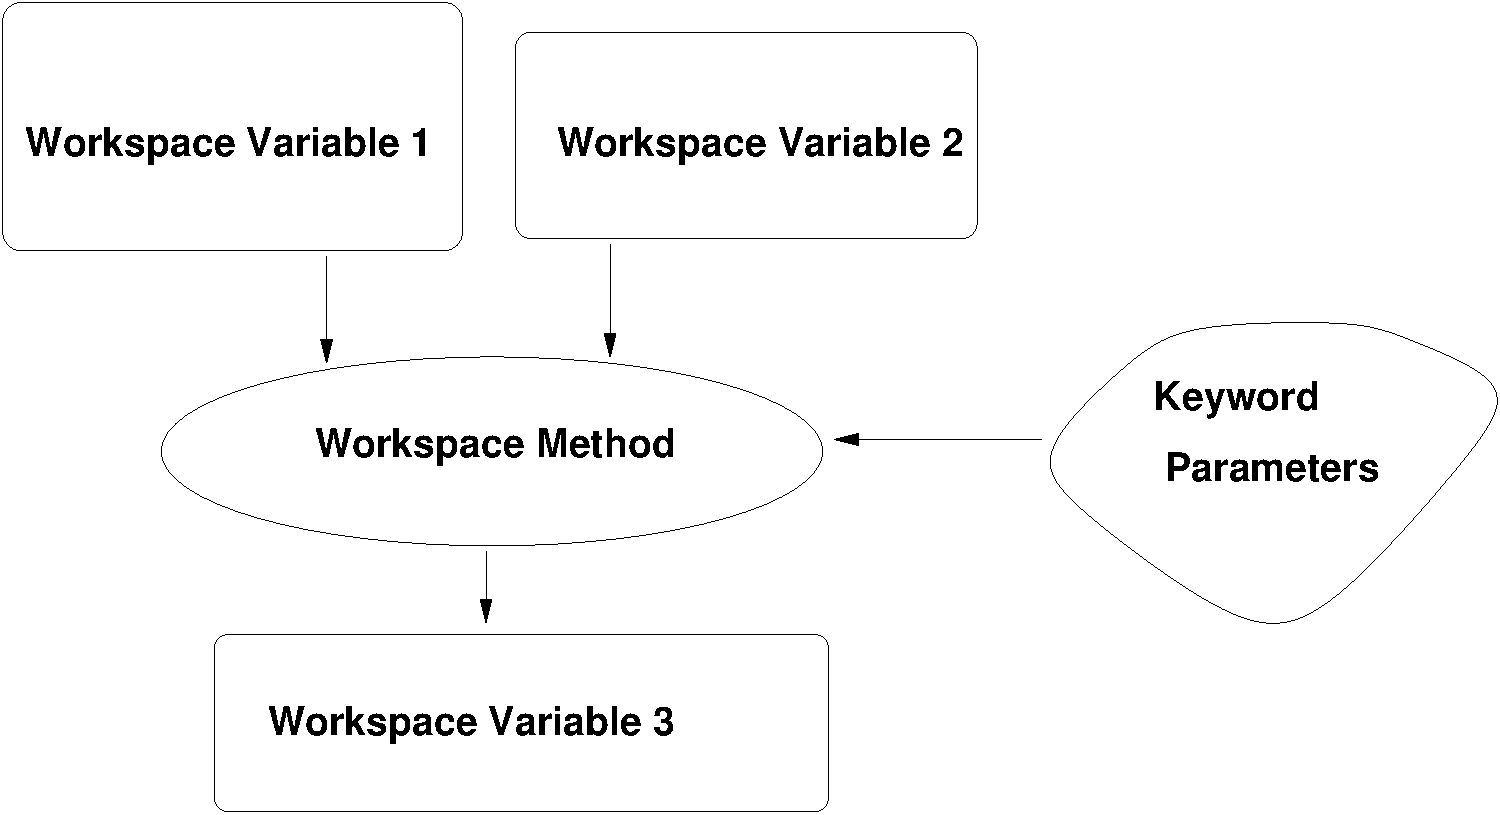
\includegraphics[width=\hsize,draft=false]{method}
    \caption{\textindex{Specific workspace methods} act on specific
      workspace variables to generate other specific workspace
      variables. Additional input parameters can be specified as
      generic input and output parameters in the control file.}
    \label{fig:method}
  \end{center}
\end{figure}

It is important to note that the control file has a fixed and
well-defined syntax. This syntax is understood by the ARTS parser.
The great advantage of this concept is that it is very easy to add
new workspace variables and new workspace methods. The program has
an internal look-up table which lists all workspace methods, as well
as their input variables, output variables, and generic input/output
parameters. To add a new method, one just has to add an entry to
this look-up table, and write the code for the method itself. No
further changes to the program are necessary. In particular, no
changes to the program logic or to the parser. How such an extension
can be made practically is described in Section \ref{sec:development}.



\subsection{Generic workspace methods}
%=================================

Generic methods (Figure \ref{fig:generic_method}) allow the user of
the program even more freedom than specific methods. A generic method
is for example \artsstyle{MatrixSetConstant}, which can be used to set any
workspace variable which is a matrix. For example
\begin{quote}
  \artsstyle{MatrixSetConstant( z\_surface, 10, 10, 0.0 )}
\end{quote}
will set the size of \artsstyle{z\_surface} to 10 x 10 where all
elements equal 0.

\begin{figure}
  \begin{center}
    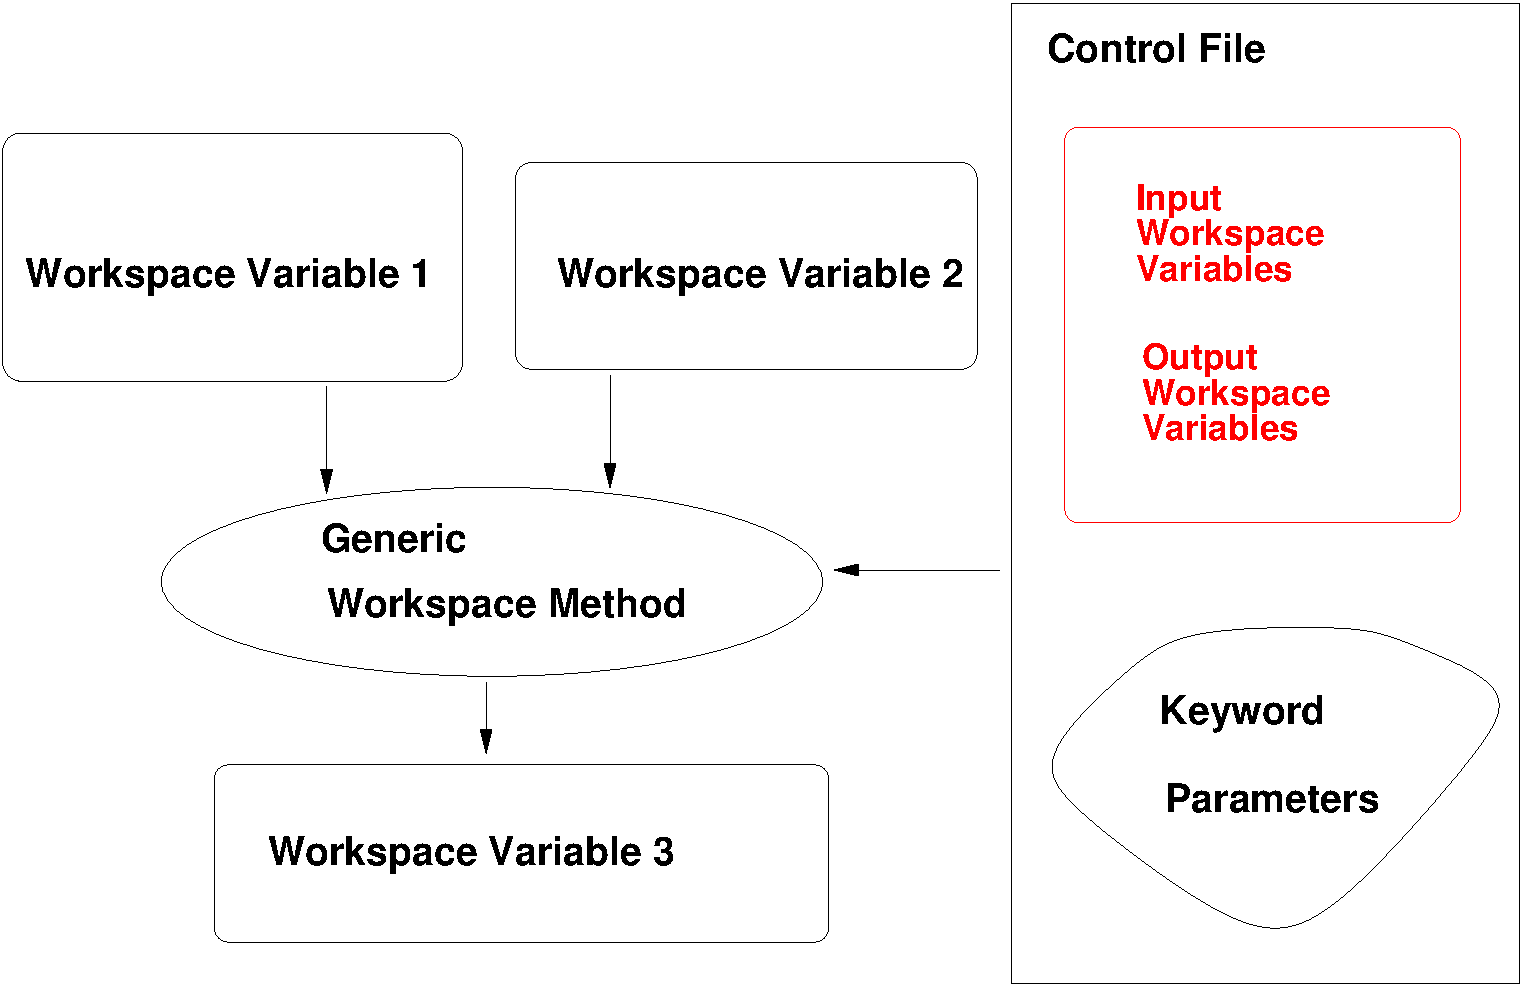
\includegraphics[width=\hsize,draft=false]{generic_method}
    \caption{For \textindex{generic workspace methods} the workspace
      variables to act on are specified in the control file.}
    \label{fig:generic_method}
  \end{center}
\end{figure}

Some methods are even more flexible, the are super generic. This means
that they can take any workspace variable as input. The most commonly
used such methods are the XML file methods. A workspace variable is
read from a file in this way
\begin{quote}
  \artsstyle{ReadXML(f\_grid,"frequency\_grid")}
\end{quote}
Generic methods are particularly useful for IO operations like in the
example above. No new IO methods are necessary for new workspace
variables, as long as they are of standard types already known to the
program (for example vectors or matrices). 



\subsection{Agendas}
%=================================

Agendas are a special incarnation of a workspace method. In the
control file an arbitrary number of workspace methods can be added to
an agenda. On invocation, the agenda executes its methods one
after the other. The inputs and outputs defined for the agenda must
be satisfied by the invoked workspace methods. E.g., if an agenda
has \artsstyle{f\_grid} in its list of output workspace variables, a
workspace method which generates \artsstyle{f\_grid} must be added to
the agenda in the control file.

Even though it is possible to execute agendas directly from the
control file with the \artsstyle{AgendaExecute} method, the more common
and intended use case is the internal invocation by other workspace
methods. This adds a grave amount of flexibility to ARTS. The
\artsstyle{RteStd} method for example calculates (besides other
components) the emission term. Without the means of an agenda, it
would only be possible to use always the same method for the emission
calculation. By the use of an agenda the user can choose between
different methods to calculate the emission and plug them into the
emission agenda in the control file:

\begin{quote}
\begin{verbatim}
AgendaSet( emission_agenda ){
  emissionPlanck
}
\end{verbatim}
\end{quote}

\noindent
\artsstyle{RteStd} internally calls the \artsstyle{emission\_agenda} and
uses the user selected method for calculating the emission term.


%%% Local Variables: 
%%% mode: latex
%%% TeX-master: "uguide"
%%% End: 
